\documentclass[twocolumn]{article}
\usepackage{amsmath, amssymb}
\usepackage[retainorgcmds]{IEEEtrantools}
\usepackage{algorithm}
\usepackage{algpseudocode}
\usepackage{filecontents}
\usepackage{hyperref}
\usepackage{graphicx}
\author{Derek Kuo, Henry Milner}
\title{CS267 Final Project: An Empirical Investigation of the Algorithmic Lov\'{a}sz Local Lemma}
\date{5/11/15}

% Some macros specific to this paper.
\newcommand{\ksat}{\texttt{k-SAT}~}

\newcommand{\polylog}{\text{polylog}}

\newcommand{\lovasz}{Lov\'{a}sz~}

% Some functions for general use.

\newcommand{\code}[1]%
  {\texttt{#1}}

\def\seqn#1\eeqn{\begin{align}#1\end{align}}

\newcommand{\vecName}[1]%
  {\boldsymbol{#1}}

\newcommand{\io}%
  {\text{ i.o. }}

\newcommand{\eventually}%
  {\text{ eventually }}

\newcommand{\tr}%
  {\text{tr}}

\newcommand{\Cov}%
  {\text{Cov}}

\newcommand{\adj}%
  {\text{adj}}

\newcommand{\funcName}[1]%
  {\text{#1}}

\newcommand{\hasDist}%
  {\sim}

\DeclareMathOperator*{\E}%
  {\mathbb{E}}

\newcommand{\Var}%
  {\text{Var}}

\newcommand{\std}%
  {\text{std}}

\newcommand{\grad}%
  {\nabla}

\DeclareMathOperator*{\argmin}{arg\,min}

\DeclareMathOperator*{\argmax}{arg\,max}

\newcommand{\inprod}[2]%
  {\langle #1, #2 \rangle}

\newcommand{\dd}[1]%
  {\frac{\delta}{\delta#1}}

\newcommand{\Reals}%
  {\mathbb{R}}

\newcommand{\indep}%
  {\protect\mathpalette{\protect\independenT}{\perp}} \def\independenT#1#2{\mathrel{\rlap{$#1#2$}\mkern2mu{#1#2}}}

\newcommand{\defeq}%
  {\buildrel\triangle\over =}

\newcommand{\defn}[1]%
  {\emph{Definition: #1}\\}

\newcommand{\example}[1]%
  {\emph{Example: #1}\\}

\newcommand{\figref}[1]%
  {\figurename~\ref{#1}}

\newtheorem{theorem}{Theorem}[section]
\newtheorem{lemma}[theorem]{Lemma}
\newenvironment{proof}[1][Proof]{\begin{trivlist}
\item[\hskip \labelsep {\bfseries #1}]}{\end{trivlist}}

\begin{filecontents}{\jobname.bib}
@article{erdos1975problems,
  title={Problems and results on 3-chromatic hypergraphs and some related questions},
  author={Erdos, Paul and Lov{\'a}sz, L{\'a}szl{\'o}},
  journal={Infinite and finite sets},
  volume={10},
  number={2},
  pages={609--627},
  year={1975}
}
@article{beck1991algorithmic,
  title={An algorithmic approach to the Lov{\'a}sz local lemma. I},
  author={Beck, J{\'o}zsef},
  journal={Random Structures \& Algorithms},
  volume={2},
  number={4},
  pages={343--365},
  year={1991},
  publisher={Wiley Online Library}
}
@article{moser2010constructive,
 author = {Moser, Robin A. and Tardos, G\'{a}bor},
 title = {A Constructive Proof of the General Lov\ÁSz Local Lemma},
 journal = {J. ACM},
 issue_date = {January 2010},
 volume = {57},
 number = {2},
 month = feb,
 year = {2010},
 issn = {0004-5411},
 pages = {11:1--11:15},
 articleno = {11},
 numpages = {15},
 url = {http://doi.acm.org/10.1145/1667053.1667060},
 doi = {10.1145/1667053.1667060},
 acmid = {1667060},
 publisher = {ACM},
 address = {New York, NY, USA},
 keywords = {Constructive proof, Lov\'{a}sz local lemma, parallelization},
} 
@article{haeupler2011new,
  title={New constructive aspects of the lovasz local lemma},
  author={Haeupler, Bernhard and Saha, Barna and Srinivasan, Aravind},
  journal={Journal of the ACM (JACM)},
  volume={58},
  number={6},
  pages={28},
  year={2011},
  publisher={ACM}
}
@inproceedings{chung2014distributed,
  title={Distributed algorithms for the Lov{\'a}sz local lemma and graph coloring},
  author={Chung, Kai-Min and Pettie, Seth and Su, Hsin-Hao},
  booktitle={Proceedings of the 2014 ACM symposium on Principles of distributed computing},
  pages={134--143},
  year={2014},
  organization={ACM}
}
@article{alon1986fast,
  title={A fast and simple randomized parallel algorithm for the maximal independent set problem},
  author={Alon, Noga and Babai, L{\'a}szl{\'o} and Itai, Alon},
  journal={Journal of algorithms},
  volume={7},
  number={4},
  pages={567--583},
  year={1986},
  publisher={Elsevier}
}
@article{luby1986simple,
  title={A simple parallel algorithm for the maximal independent set problem},
  author={Luby, Michael},
  journal={SIAM journal on computing},
  volume={15},
  number={4},
  pages={1036--1053},
  year={1986},
  publisher={SIAM}
}
@inproceedings{freer2010probabilistic,
  title={When are probabilistic programs probably computationally tractable?},
  author={Freer, Cameron E and Mansinghka, Vikash K and Roy, Daniel M},
  booktitle={NIPS Workshop on Advanced Monte Carlo Methods with Applications},
  year={2010}
}
@article{wainwright2008graphical,
  title={Graphical models, exponential families, and variational inference},
  author={Wainwright, Martin J and Jordan, Michael I},
  journal={Foundations and Trends{\textregistered} in Machine Learning},
  volume={1},
  number={1-2},
  pages={1--305},
  year={2008},
  publisher={Now Publishers Inc.}
}
@inproceedings{papadimitriou1991selecting,
  title={On selecting a satisfying truth assignment},
  author={Papadimitriou, Christos H},
  booktitle={Foundations of Computer Science, 1991. Proceedings., 32nd Annual Symposium on},
  pages={163--169},
  year={1991},
  organization={IEEE}
}
@article{peleg2000distributed,
  title={Distributed computing},
  author={Peleg, David},
  journal={SIAM Monographs on discrete mathematics and applications},
  volume={5},
  year={2000},
  publisher={Springer}
}
@inproceedings{steurer2010fast,
  title={Fast SDP algorithms for constraint satisfaction problems},
  author={Steurer, David},
  booktitle={Proceedings of the twenty-first annual ACM-SIAM symposium on Discrete Algorithms},
  pages={684--697},
  year={2010},
  organization={Society for Industrial and Applied Mathematics}
}
@inproceedings{polik2007sedumi,
  title={SeDuMi: a package for conic optimization},
  author={Polik, Imre and Terlaky, Tamas and Zinchenko, Yuriy},
  booktitle={IMA workshop on Optimization and Control, Univ. Minnesota, Minneapolis},
  year={2007}
}
@article{malaguti2010survey,
  title={A survey on vertex coloring problems},
  author={Malaguti, Enrico and Toth, Paolo},
  journal={International Transactions in Operational Research},
  volume={17},
  number={1},
  pages={1--34},
  year={2010},
  publisher={Wiley Online Library}
}
@inproceedings{coja2014asymptotic,
  title={The asymptotic k-sat threshold},
  author={Coja-Oghlan, Amin},
  booktitle={Proceedings of the 46th Annual ACM Symposium on Theory of Computing},
  pages={804--813},
  year={2014},
  organization={ACM}
}

@article{gomes2008satisfiability,
  title={Satisfiability solvers},
  author={Gomes, Carla P and Kautz, Henry and Sabharwal, Ashish and Selman, Bart},
  journal={Foundations of Artificial Intelligence},
  volume={3},
  pages={89--134},
  year={2008},
  publisher={Elsevier}
}
@article{balint2013generating,
  title={Generating the uniform random benchmarks for SAT Competition 2013},
  author={Balint, Adrian and Belov, Anton and Heule, Marijn JH and J{\"a}rvisalo, Matti},
  journal={Proceedings of SAT Competition},
  pages={97--98},
  year={2013}
}
@article{belov2014application,
  title={The Application and the Hard Combinatorial Benchmarks in SAT Competition 2014},
  author={Belov, Anton and Heule, Marijn JH and Diepold, Daniel and J{\"a}rvisalo, Matti},
  journal={SAT COMPETITION 2014},
  pages={81}
}

@article{belov2014sat,
  title={SAT COMPETITION 2014},
  author={Belov, Anton and Diepold, Daniel and Heule, Marijn JH and J{\"a}rvisalo, Matti},
  year={2014}
}

\end{filecontents}
\immediate\write18{bibtex \jobname}

\begin{document}
\maketitle

\begin{abstract}
The algorithmic \lovasz Local Lemma (LLL) is a recent-developed meta-algorithm for solving certain instances of hard combinatorial problems.  In theory, LLL algorithms can be applied whenever a problem can be decomposed into smaller subproblems and the dependencies among subproblems are, in a certain sense, somewhat sparse.  For example, a \ksat problem can be decomposed into the problem of satisfying each of its clauses, and LLL algorithms can be useful in solving \ksat problems whose clauses do not share literals with too many other clauses.  The seminal paper in the field is by Moser and Tardos \cite{moser2010constructive} in 2010.  For many problems, LLL algorithms theoretically lend themselves well to parallelism, as demonstrated in \cite{moser2010constructive} and expanded upon in more recent work \cite{chung2014distributed,haeupler2011new} that focuses in particular on distributed algorithms.  However, we are aware of no published empirical tests of the efficiency of LLL algorithms in practice; the existing literature focuses entirely on proving results about their asymptotic performance.  In this paper, we give concrete implementations of serial and distributed LLL algorithms for \ksat, and we give a preliminary evaluation of their performance.
\end{abstract}

\section{Introduction}
\label{sec:intro}
In 1975, Erd\"{o}s and \lovasz \cite{erdos1975problems} developed a technique, now called the \lovasz Local Lemma (LLL), for proving the existence of solutions to combinatorial problems.  The technique is a ``probabilistic method'': Given a set of events that we want to avoid (for example, each event could correspond to the violation of one problem constraint), it is proved that there is a strictly positive probability that none of these events if we draw randomly from a suitable distribution on potential solutions.  The main precondition of the LLL is that the statistical dependencies among events are \emph{sparse}, with the sparsity being of the same magnitude as the marginal probability of each single event being unsatisfied under the sampling distribution.  We will discuss the technique later in more detail.

For many years the LLL was viewed as a tool useful only in proofs.  In 1991, Beck \cite{beck1991algorithmic} found randomized algorithms for several combinatorial problems that actually \emph{find} solutions, and which finish in expected polynomial time under conditions similar to the preconditions of the LLL.  The CS theory community continued to improve on these results, until in 2010 Moser and Tardos \cite{moser2010constructive} published a meta-algorithm for solving, in expected polynomial time, any combinatorial problem that satisfies the LLL preconditions.

An interesting aspect of the Moser-Tardos meta-algorithm is that it can be parallelized.  Moser and Tardos analyzed a simple parallel version of their algorithm in their original paper.  More recently, Chung et al \cite{chung2014distributed} and Haeupler et al \cite{haeupler2011new} developed algorithms requiring less communication in a distributed environment.  All of these algorithms finish in $\tilde{O}(1)$ time given a number of processors that grows linearly with the problem description length.  However, the big-$\tilde{O}$ hides logarithmic factors and potentially large constants.

Though they seem promising, to our knowledge neither the Moser-Tardos meta-algorithm nor its parallel variants have ever been tested empirically.  Several questions of practical interest are left open by the existing literature:
\begin{enumerate}
  \item When the preconditions of the LLL are satisfied, does the Moser-Tardos meta-algorithm actually run quickly, or does the analysis hide large constant factors?
  \item Under those conditions, is the Moser-Tardos meta-algorithm competitive with existing solvers for hard combinatorial problems?
  \item Are there interesting and difficult problems that satisfy the preconditions of the LLL?
  \item Are the preconditions of the LLL actually necessary in practice for the Moser-Tardos meta-algorithm to work efficiently?  How quickly does its performance degrade as the preconditions become more unsatisfied?
  \item Are the parallel LLL algorithms useful in practice?
\end{enumerate}

In this paper, we study only the last question: Are the parallel LLL algorithms useful in practice?  In particular, we consider algorithms designed for \emph{distributed-memory} systems (though shared-memory parallelism and GPUs would both be interesting future directions).  In order to answer our question it will be necessary to give partial answers to the others, but we leave more thorough investigations for future work.

To study applications of the algorithmic LLL, we must choose a combinatorial problem to solve.  We focus on \ksat.  In \ksat, we are given $n$ boolean variables and $m$ disjunctive (``OR'') clauses of $k$ possibly-negated variables each, and we must find an assignment of the variables that satisfies all of the clauses.  The decision version of \ksat is NP-complete, but this does not necessarily mean that instances of practical importance (or, possibly, all but a small number of worst-case instances) are hard, and there is a long and ongoing history of work on heuristic search methods for the problem.  In fact, there is an annual competition for SAT solvers \cite{belov2014sat}.  (Our benchmarks will be based on the guidelines in that competition.)  We do not expect that our implementations will be competitive with state-of-the-art SAT solvers, and such comparisons are outside the scope of this project.  Our interest is primarily in finding out whether there is any practical potential for an algorithm whose development has thus far been guided exclusively by the desire to prove results about its performance.

Our main contribution is a collection of serial and distributed implementations of LLL algorithms for \ksat.  Our serial code is written in Julia, and our distributed code is written in Python, using MPI via the mpy4py library.  All code is available at \texttt{https://github.com/henryem/lll} .

\subsection{This Paper}
In section \ref{sec:alll}, we discuss in detail the Moser-Tardos meta-algorithm.  In section \ref{sec:implementation}, we describe our implementation of particular forms of the algorithm and the design choices we made.  In section \ref{sec:benchmarks} we comment on the design of benchmarks, which is nontrivial for \ksat.  In section \ref{sec:scaling}, we present scaling results for our chosen benchmarks.  We conclude in section \ref{sec:discussion} with a discussion of our results and directions for future work.

\section{The Algorithmic \lovasz Local Lemma}
\label{sec:alll}
LLL algorithms can be useful for problems that can be phrased as follows.  Let $\mathcal{A} = \{A_1, \cdots, A_n\} \in \{0,1\}^n$ be a set of discrete variables (which we take to be binary for sake of exposition), and let $\mathcal{E} = \{E_1, \cdots, E_m\}$ be a set of functions $\{0,1\}^n \to \{0,1\}$ mapping the variables to truth values.  The $E_i$ are called ``events,'' and $E_i$ is said to ``happen'' under some assignment to $\mathcal{A}$ if $E_i(\mathcal{A}) = 1$.  We would like to find an assignment of the variables so that none of the events happen.

This framework encompasses many constraint satisfaction problems.  For example, we can encode graph coloring as follows: the variables are binary encodings of the color assignments to vertices, and event $E_{ij}$ happens if vertices $i$ and $j$ are assigned the same color.  Then if we find an assignment of the variables for which none of the events happen, we have found a graph coloring.  Encoding \ksat is even more straightforward: the $A_i$ are the problem variables, and each $E_i$ corresponds to a clause involving $k$ variables.  $E_i$ happens if the corresponding clause is false, and an assignment solves the problem if none of the events happen.  In \ksat, each event $E_i$ is a function of only a smaller subset of the variables (of size $k$), and it is functionally independent of the rest.  We denote that subset of $\mathcal{A}$ by $\operatorname{vbl}(E_i)$.  If we imagine randomly and independently determining the variable values, then $E_i$ is statistically dependent only on $\operatorname{vbl}(E_i)$.  LLL algorithms typically need $|\operatorname{vbl}(E_i)| \ll |\mathcal{A}|$.

\subsection{The Moser-Tardos meta-algorithm}
The simplest LLL algorithm, the Moser-Tardos meta-algorithm, is \emph{extremely} simple.  It is algorithm 1 below.  Its specialization to \ksat is algorithm 2.

\begin{algorithm}[H]
\label{alg:mt-meta}
\begin{algorithmic}[1]
\State Initialize all the $A_i$ as i.i.d. samples from a uniform Bernoulli distribution.
\While{Any of the $E_j$ happen under the current value of $\mathcal{A}$}
  \State Let $E_j$ be an arbitrary event that happens under $\mathcal{A}$.
  \State Resample each $A_i \in \operatorname{vbl}(E_j)$ i.i.d. uniform Bernoulli.
\EndWhile
\end{algorithmic}
\caption{The Moser-Tardos meta-algorithm.}
\end{algorithm}

\begin{algorithm}[H]
\label{alg:mt-ksat}
\begin{algorithmic}[1]
\State Initialize all variables $V_i$ as i.i.d. samples from a uniform Bernoulli distribution.
\While{Any clause is violated}
  \State Let $C_j$ be an arbitrary clause that is violated.
  \State Resample each $V_i \in \operatorname{vbl}(C_j)$ i.i.d. uniform Bernoulli.
\EndWhile
\end{algorithmic}
\caption{The Moser-Tardos meta-algorithm, specialized to \ksat.}
\end{algorithm}

\begin{figure}[ht]
  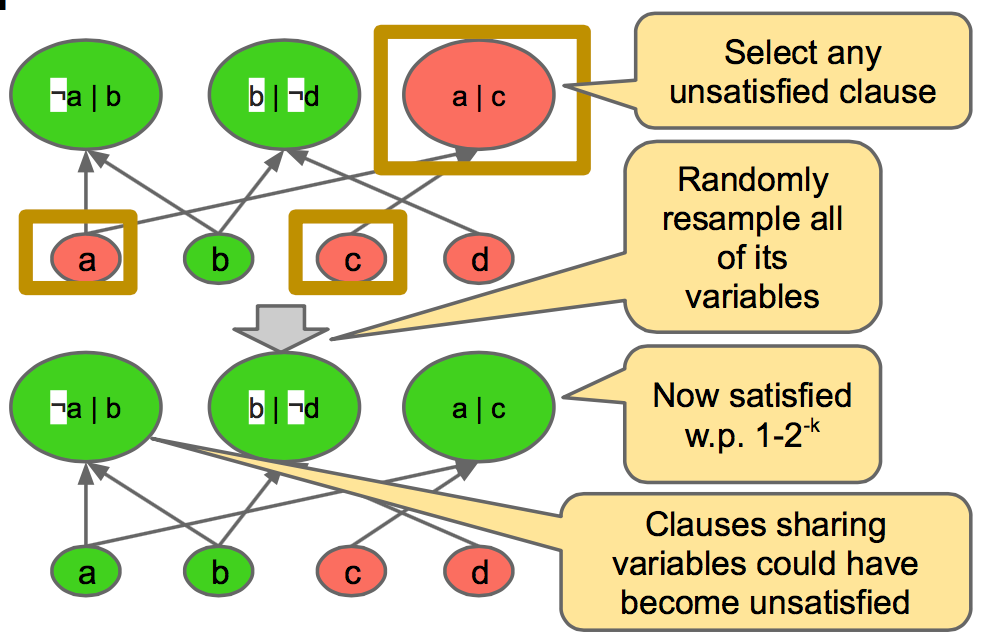
\includegraphics[scale=0.5]{figures/mt-directed-example.png}
  \caption{One iteration of an example run of the Moser-Tardos meta-algorithm for \ksat.  The problem is $(!a|b)\&(b|!d)\&(a|c)$.  The variables $a$, $b$, $c$, and $d$ are initialized uniformly at random before the algorithm starts.}
  \label{fig:mt-directed-example}
\end{figure}

To illustrate the algorithm, it helps to associate an LLL problem with a bipartite \emph{directed probabilistic graph} (sometimes also called a \emph{Bayes' net}).  Each variable and each event is a node in this graph, and there is a directed edge from each variable to each event that depends on it.  (The events are deterministic given the variables, but in a randomized algorithm the process that generates the variable values is random.)  Figure \ref{fig:mt-directed-example} shows an example run of the Moser-Tardos meta-algorithm for a \ksat problem through the lense of this directed graph.

Of course, the decision version of \ksat is NP-hard, so we would not expect this algorithm to work well for all instances.  Moser and Tardos \cite{moser2010constructive} prove that it runs in expected polynomial time when the events are not individually too hard to satisfy with random assignment and when there are not too many dependencies among the events.

To make this concrete, it is useful to associate another graph with an LLL problem: its dependency graph.  This is an undirected graph in which each event is a node, and in which there is an edge between events $E_j$ and $E_k$ if they are statistically dependent under independent random assignment to the $A_i$, or equivalently if any variable in the directed probablistic graph points to both $E_j$ and $E_k$.  In \ksat, there is an edge between clauses $E_j$ and $E_k$ if they share any variable.  Figure \ref{fig:mt-undirected-example} has an example dependency graph for the problem pictured in figure \ref{fig:mt-directed-example}.

\begin{figure}[ht]
  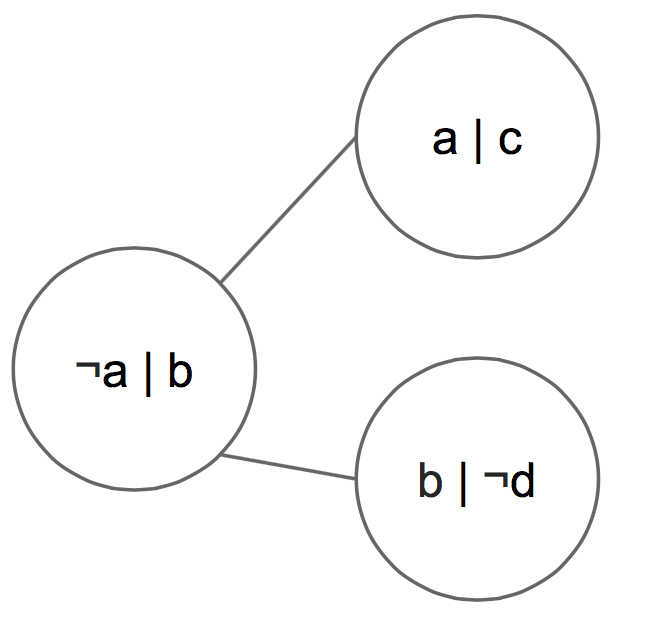
\includegraphics[scale=0.5]{figures/mt-undirected-example.png}
  \caption{The dependency graph for the problem pictured in figure \ref{fig:mt-directed-example}.}
  \label{fig:mt-undirected-example}
\end{figure}

Let $d$ be the maximum degree of events in the dependency graph for a problem instance.  And let $p$ be the maximum probability that any single event happens under a uniform random assignment to all the variables.  In \ksat, $p = 2^{-k}$, since a disjunctive clause is unsatisfied only if all of its k variables are assigned incorrectly, and the single variable assignments happen independently with probability $1/2$.  Then Moser and Tardos prove that algorithm 1 finishes in expected polynomial time if $e p d < 1$, where $e$ is the base of the natural logarithm.  These are the same conditions under which the ordinary \lovasz Local Lemma guarantees the \emph{existence} of a solution.

A \ksat problem satisfies this condition if each clause shares variables with no more than $\frac{2^k}{e}$ other clauses.  For instance, if we generate a random \ksat instance with $n$ variables and $m$ clauses (and random signs), the probability that two clauses share a variable is approximately $\frac{k^2}{n}$, so the expected degree of any node is approximately $\frac{m k^2}{n}$.  If we make the optimistic assumption that the maximum degree equals the expected degree, then the proof by Moser and Tardos applies if $m$ is less than $\frac{2^k n}{k^2 e}$.  For comparison, the maximum number of clauses in a \ksat instance is $2^k {n \choose k}$.  It is known that random 3-SAT instances are hardest when $m \approxeq 4.26 n$ \cite{gomes2008satisfiability}, so these are relatively easy instances.  In fact, for $k = 3$ these instances do not even use all the variables, since $\frac{2^3 m}{3^2 e} = \frac{8}{9e} < 1/3$.  For larger $k$, the instances for which the proof by Moser and Tardos applies can be much less trivial than that, but they can never meet the threshold, which is asymptotically $(\log 2) 2^k - \frac{1}{2}(1 + \log 2)$\cite{coja2014asymptotic}.  Of course, we should not expect to be able provably to solve hard instances of NP-complete problems in polynomial time!  We will provide empirical results for problems that are at varying degrees of proximity to the hardness threshold.

\subsection{Parallelizing Moser-Tardos}
The event dependency graph is useful for seeing a way to parallelize algorithm 1.  Notice that if independent events $E_j$ and $E_k$ happen under the current assignment to $\mathcal{A}$, and event $E_j$'s variables are chosen for resampling, then (by independence) $E_k$ will still happen after the resampling, so there exists a valid serial execution of the algorithm in which the next iteration resamples $E_k$'s variables.  This means we can resample variables depended-on by any independent set of events that currently happen, and this resampling can be done in parallel.  Figure \ref{fig:mt-independence-example} gives an example.

\begin{figure}[ht]
  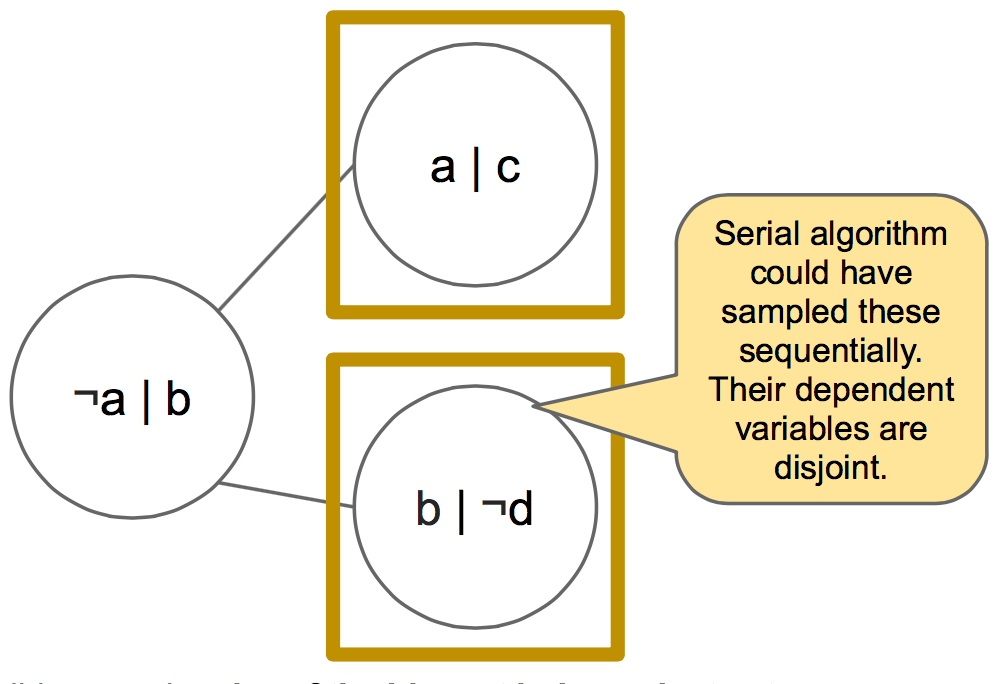
\includegraphics[scale=0.4]{figures/mt-independence-example.png}
  \caption{The dependency graph for the problem pictured in figure \ref{fig:mt-directed-example}, with an independent set highlighted.  If these two clauses are unsatisfied at some stage of the algorithm, the variables of both can be resampled simultaneously.  If we could only identify a smaller independent set, there would be less opportunity for parallelism.}
  \label{fig:mt-independence-example}
\end{figure}

The larger the independent set we can find, the more parallelism is available.  In fact, Moser and Tardos prove that the algorithm terminates in $O(\log(m))$ iterations -- that is, it has sub-linear computational depth -- if the variables of a \emph{maximal} independent set are resampled at each step.  (Note that the requirement is not for a \emph{maximum} independent set, finding which is itself an NP-complete problem, but merely an independent set that cannot be greedily extended.)  Since the set of events that happen changes on each iteration, it is necessary to find new independent sets on each iteration, so this is not a fixed cost.  In practice, this is a major bottleneck of the algorithm.  Moser and Tardos suggest using Luby's algorithm \cite{luby1986simple}.  In short, that algorithm grows an independent set by assigning random IDs to each node in the graph, then iteratively adding all remaining strict local minima to the independent set, and removing the added nodes and their neighbors.  It finds a maximal independent set using $O(\log m)$ rounds of communication and $O(m \log m)$ total work, in expectation and with high probability.  Chung et al \cite{chung2014distributed} and Srinivasan et al \cite{haeupler2011new} give alternative parallel LLL algorithms that can be run more efficiently on distributed computers.  These algorithms differ only in the methods they use to find independent sets; the requirement for a maximal independent set is typically relaxed in some fashion.

For our parallel code, we have implemented the so-called ``simple'' algorithm of Chung et al (algorithm 2 in \cite{chung2014distributed}) using some techniques suggested by Haeupler et al \cite{haeupler2011new}.  We call this algorithm 3, and pseudocode is given below.

\begin{algorithm}[H]
\label{alg:chung-simple}
\begin{algorithmic}
\State Initialize all the $A_i$ as i.i.d. samples from a uniform Bernoulli distribution.
\State Mark each of the $E_j$ with a random integer ID.
\While{Any of the $E_j$ happen under the current value of $\mathcal{A}$}
  \State Let $U = \{E_j: E_j\text{ currently happens}\}$. 
  \State Let $S = \{E_j: E_j \in U, ID(E_j) < \min_{k \in \Gamma(j) \cap U} ID(E_k)\}$, the set of strict local minima among unsatisfied events.
  \State Resample each $A_i \in \cup_{E_j \in S} \operatorname{vbl}(E_j)$ i.i.d. uniform Bernoulli.
\EndWhile
\end{algorithmic}
\caption{The ``simple'' algorithm of Chung et al.  Here $\Gamma(j)$ is the set of neighbors of event $E_j$ in the dependency graph.}
\end{algorithm}

Algorithm 3 simply uses Luby's algorithm, but stops after a single iteration rather than continuing until a maximal independent set has been found.  Further, the random IDs are reused across iterations of algorithm 1.  We will see that these two modifications substantially reduce the communication requirements of the Moser-Tardos meta-algorithm.  The pseudocode does not address the parallelism or communication patterns used in the algorithm, which is the subject of section \ref{sec:implementation}.  It should be noted, however, that algorithm 3 is proven to run in polynomial time only when $e p d^2 < 1$, a stronger requirement.  Chung et al provide another algorithm with the same dependency on $d$ as the Moser-Tardos meta-algorithm (algorithm 3 in their paper), but it involves more communication than the simple algorithm.  We implemented only a serial version of it.

% Last, it should be noted that the simple LLL algorithm is quite similar to stochastic local search heuristics for \ksat that have been known for many years.  It would be surprising if it performed much better than those older methods, or the more sophisticated heuristics that have followed them.  So we expect to find negative results.  The parallel LLL algorithms are less obvious, so there is more hope that they outperform or outscale existing algorithms on instances that satisfy Moser's condition for efficiency.

\section{Our Implementation}
\label{sec:implementation}
We have written Julia implementations of algorithms 2 and 3, and algorithm 3 in \cite{chung2014distributed}.  Each of these algorithms is a modification of the Moser-Tardos meta-algorithm with a particular way of finding independent sets.  Since there is potentially a tradeoff between the time spent to find independent sets and the number of iterations the algorithm must perform, these implementations are useful for independently examining the number of iterations taken by each algorithm.  Otherwise, since it is serial, the Julia code is straightforward. 

We have also written a Python implementation of algorithm 3 using the MPI bindings in the mpi4py library.  Since this code is targeted at a distributed-memory environment, we had to consider how to parallelize each step of the algorithm.  We made rather different design choices than suggested by Chung et al.

Chung et al assume the LOCAL model of communication \cite{peleg2000distributed}.  In this model, each clause of the \ksat problem is assigned its own processor and may communicate with its neighbors in the dependency graph.  The running time of an algorithm in this model is proportional to the number of communication rounds.  Since a clause's variables are shared only with its neighbors in the dependency graph, variable updates need only be shared among neighbors.  And Luby's algorithm for independent sets only requires nodes to communicate with their neighbors to discover whether any are currently unsatisfied and have smaller IDs.  In principle, we could use this as a recipe for our code.  In practice, however, using one processor per clause is tremendously wasteful of computational resources.  It would be practical only for very small problems that could be more efficiently solved serially.

Instead, we assume that responsibility for the clauses is divided among a small number of processors $p$.  Specifically, we assume that the number of processors is small enough, and the dependency graph dense enough, that at least one edge will cross between the subgraphs of the dependency graph on each processor, with high probability.  (This assumption holds true even for the easiest \ksat instances we use in our benchmarks.)  This leads to several design decisions:
\begin{enumerate}
  \item When computing independent sets, each processor may need to check the satisfiedness of every problem clause in order to determine whether its own clauses are local minima in the dependency graph.  To accomplish this, we could compute the satisfiedness of every clause in parallel and then broadcast them.  But this involves $O(m)$ communication per iteration, which is more expensive than simply computing it each machine at a cost of $O(m)$ computation.  So we initially broadcast all of the the problem clauses to each processor, and after initialization, each processor can compute satisfiedness of any clause given an up-to-date assignment to the variables.
  \item The processor responsible for each clause must identify its neighbors in the dependency graph.  This involves a scan that takes $O(m^2)$ work (though a more sophisticated algorithm that is harder to parallelize takes $O(m k)$ work).  However, given that all the clauses have been broadcast to every processor, this step is embarrassingly parallel.
  \item Our assumption on $p$ implies that each processor has at least one clause that depends on each variable, with high probability.  Therefore the variable assignments must be broadcast across the clusters on each iteration, at the cost of one phase of $O(n)$ communication.
  \item With the above two choices, the only coupling among the nodes is the variable assignments.  All other computation proceeds independently, and the variable broadcast is the only communication required (other than the startup cost of broadcasting the clauses).
\end{enumerate}

Algorithm 4 gives pseudocode for our implementation.

\begin{algorithm}[H]
\label{alg:implementation}
\begin{algorithmic}
\State Broadcast all clauses.
\State Assign each clause to a processor $p(j)$.
\State For each clause $j$, compute the neighbor set $\Gamma(j)$ on processor $p(j)$.
\State Mark each clause with a random integer ID, and broadcast these marks.
\State Broadcast an initial random assignment of the variables.
\While{True}
  \State Let $U_k$ be the set of violated clauses assigned to processor $k$.
  \State Let $U$ be the set of all violated clauses, constructed lazily on each processor.
  \State Let $S_k = \{E_j: E_j \in U_k, ID(E_j) < \min_{k \in \Gamma(j) \cap U} ID(E_k)\}$.
  \State Let $V_k = \cup_{E_j \in S_k} \operatorname{vbl}(E_j)$.
  \State On each processor $k$, resample each variable in $V_k$.
  \State Broadcast the new variable assignments.
  \State Terminate if no new variables have been assigned anywhere.
\EndWhile
\end{algorithmic}
\caption{The ``simple'' algorithm of Chung et al, as we have implemented it.}
\end{algorithm}

\section{Benchmarking \ksat}
\label{sec:benchmarks}
Ideally we would use real problems to test our implementation.  Since \ksat is NP-complete, there are surely instances that will take exponential time, and there is no complete theoretical characterization of these instances to guide our selection of synthetic instances.  Unfortunately, due to time constraints we are forced to leave real problems for future work.

Instead, we focus on randomly-generated synthetic instances.  A randomly-generated \ksat instance with parameters $m$, $n$, and $k$ has $m$ clauses, each of which selects one of the ${n \choose k}$ subsets of $k$ variables uniformly at random.  Each variable in each clause is negated with probability $1/2$.  It is important to be careful about the selection of problem parameters, since many choices lead to uninteresting problems.  If $m$ is too small, most variable assignments will solve most instances, while if $m$ is too large, most instances will be unsatisfiable.  The annual SAT competition \cite{belov2014sat} provides some guidance on the choice of $m$, $n$, and $k$, and our parameter choices are similar to those in the 2009 competition.  However, it is still unclear how to characterize the difficulty of a particular random instance.  Even with parameters that typically generate hard problems, some instances will be easy or impossible.  To generate our benchmarks, we use rejection sampling to find instances for which no more than a small fraction of assignments solve the instance, taking this as our proxy for problem difficulty.

\section{Results}
\label{sec:scaling}
We perform all of our experiments on the Hopper cluster.

\subsection{Strong scaling and profiling}
Strong scaling for one instance is displayed in figure \ref{fig:strong}.  The algorithm scales almost perfectly for this large problem.  Profiling our code, we found to our surprise that the initial neighbor identification stage was the primary bottleneck.  This involves iterating over each pair of nodes and is embarrassingly parallel, so it takes $O(m^2/p)$ time, where $p$ is the number of processors used.  This explains the favorable scaling.  Profiling results are displayed in figures \ref{fig:profiling} and \ref{fig:profiling-strong}.

\begin{figure}[ht]
  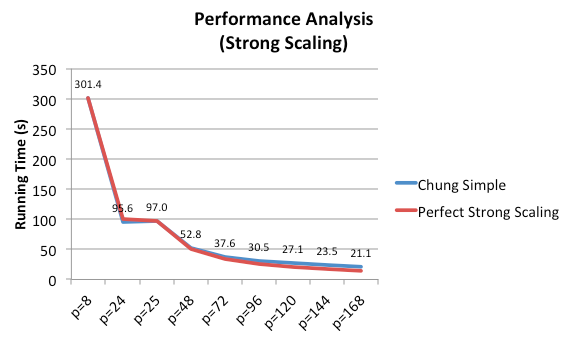
\includegraphics[scale=0.4]{figures/strong.png}
  \caption{Strong scaling for a large problem.}
  \label{fig:strong}
\end{figure}

\begin{figure}[ht]
  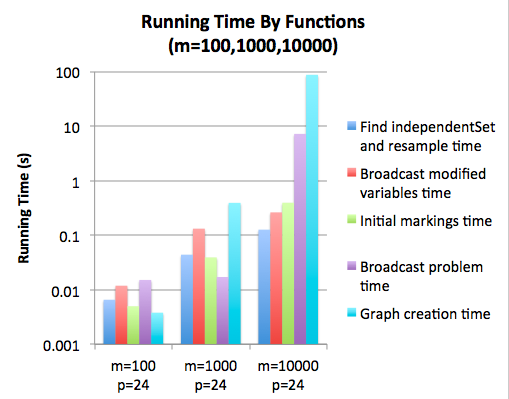
\includegraphics[scale=0.4]{figures/profiling.png}
  \caption{Profiling results for varying problem sizes, in log scale.}
  \label{fig:profiling}
\end{figure}

\begin{figure}[ht]
  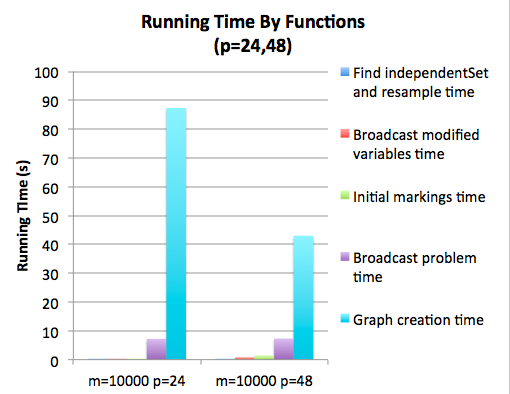
\includegraphics[scale=0.4]{figures/profiling-strong.png}
  \caption{Profiling results for a large problem using 1 and 2 Hopper nodes.}
  \label{fig:profiling-strong}
\end{figure}

\subsection{Weak scaling}
For the reasons described in section \ref{sec:benchmarks}, weak scaling is difficult to establish, since the difficulty of a problem is not simple to define.  We attempted to use as a proxy for problem difficulty the probability that a random assignment to the variables would solve the problem.  This proxy was reasonable for small problems, but unreasonable for large ones.  Figure \ref{fig:weak} displays the results of this test.  It appears from this figure that the algorithm scales worse than linearly even as $p$ increases linearly with $m$, but this is likely an artifact of our poor proxy for problem difficulty.  Strong scaling seems to be a more meaningful measure of the utility of parallelism for this problem.

\begin{figure}[ht]
  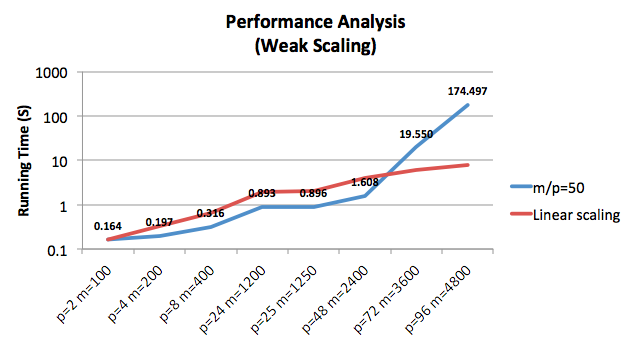
\includegraphics[scale=0.4]{figures/weak.png}
  \caption{An attempted experiment to demonstrate weak scaling.  Large problems are much harder than our proxy suggests.}
  \label{fig:weak}
\end{figure}

\subsection{The LLL condition}
All theoretical results for algorithm 4 require the condition $e p d^2 < 1$, as discussed above.  Theoretical results for other LLL algorithms require $e p d < 1$.  However, in our benchmarks we observe no such hard requirement, nor a threshold effect at $e p d \approxeq 1$.  Figure \ref{fig:lll-condition} compares the number of iterations taken to solve an instance with the value of $e p d$.  There is no noticeable change at $e p d = 1$.  This suggests that there may be room for improvement in the theoretical results.

\begin{figure}[ht]
  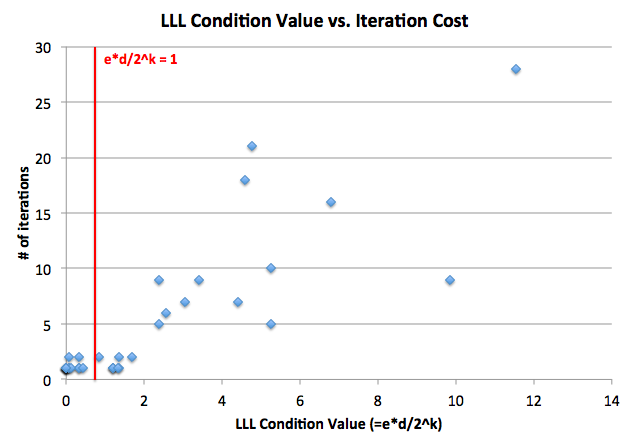
\includegraphics[scale=0.4]{figures/lll-condition.png}
  \caption{The LLL condition value of a problem ($e p d$) versus the number of iterations taken by algorithm 3.  The problems become harder as $e p d$ increases, but there is no sharp threshold at $1$.}
  \label{fig:lll-condition}
\end{figure}

\section{Discussion}
\label{sec:discussion}
Overall, our results are positive.  Algorithm 4 performs quite well on the range of problems we have tested, and it exhibits strong scaling.  By naive random search, we could find no cases in which a problem has a satisfying solution that could not be found in fewer than a hundred iterations of algorithm 4.  The current bottleneck, neighbor identification, is embarrassingly parallel.

In addition to the questions enumerated in section \ref{sec:intro}, our results leave several open questions for future work:
\begin{description}
  \item[Neighbor identification:] Can we speed up neighbor identification?  An initial random assignment of all variables will satisfy, on average, all but $m 2^{-k}$ clauses, and many clauses may never be unsatisfied during a run of the algorithm.  If we computed neighbor sets lazily, we could avoid doing any work for these always-satisfied clauses, potentially reducing the cost of neighbor identification by a factor of $2^k$.
  \item[GPUs:] Our implementation targets a distributed-memory environment, but GPUs could be better choices.  In a GPU, an implementation closer to the LOCAL computational model, with $p \approxeq m$, might be appropriate.
\end{description}

\bibliographystyle{plain}
\bibliography{\jobname}

\end{document}